\documentclass{article}

\usepackage{graphicx}
\usepackage{tikz}
\usepackage{tikzsymbols}
\usetikzlibrary{calc,patterns,shapes.geometric}
\pagestyle{empty}
\usepackage[margin=0pt]{geometry}
\geometry{papersize={14in,12in}}

\def\centerarc[#1](#2)(#3:#4:#5){\draw[#1] ($(#2)+({#5*cos(#3)},{#5*sin(#3)})$) arc (#3:#4:#5);}

\begin{document}
	\begin{figure}
		\centering
		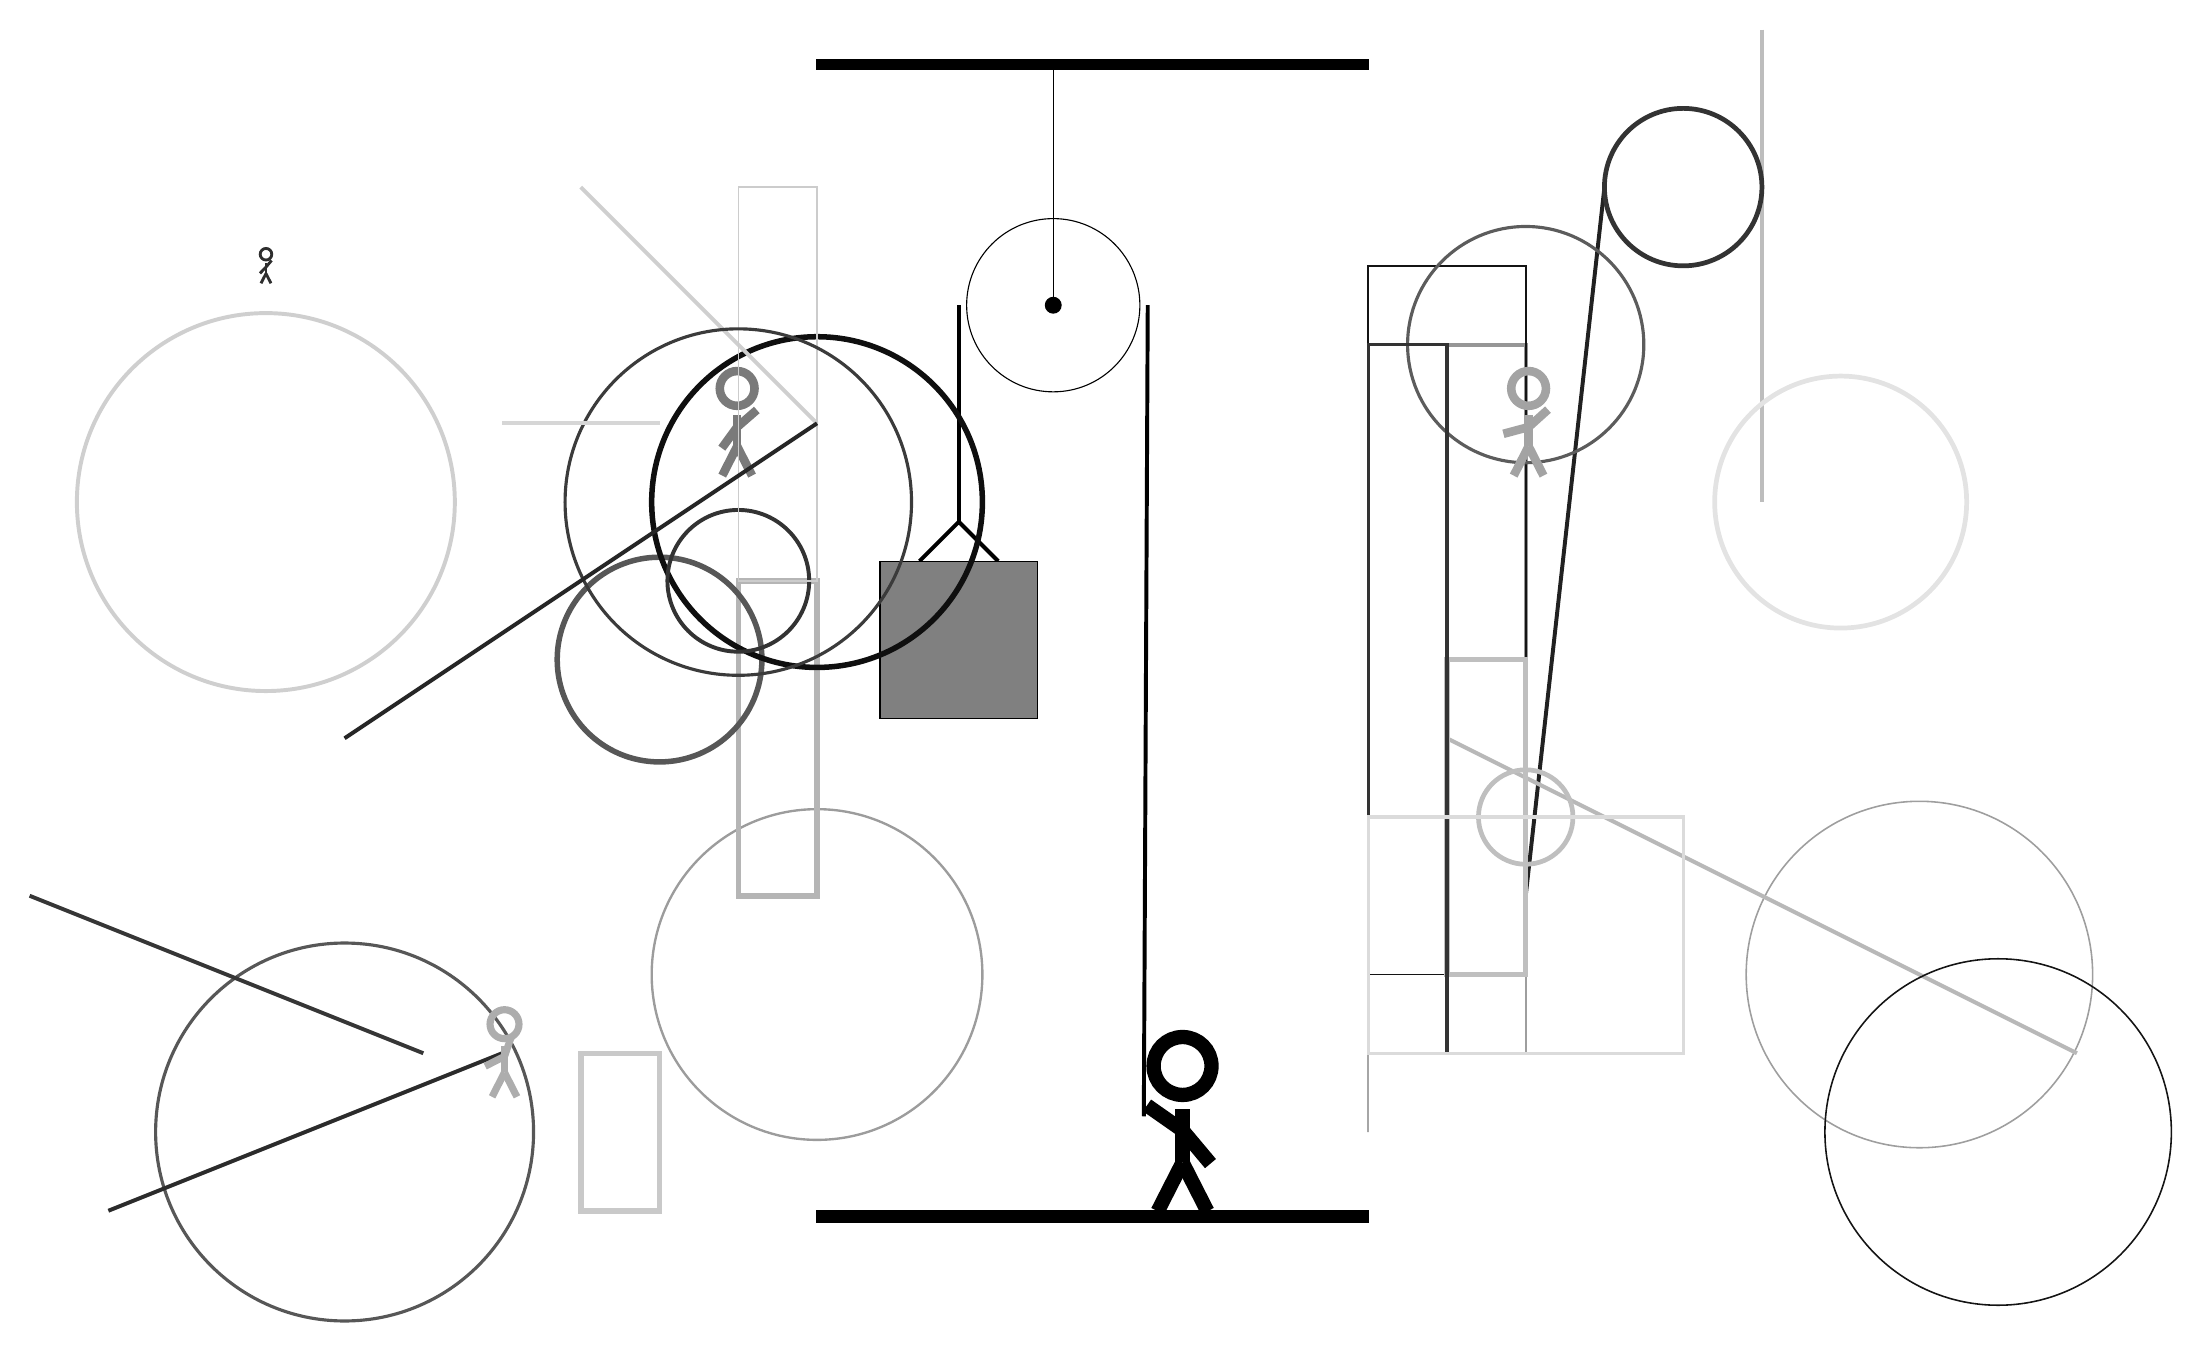
\begin{tikzpicture}
			%%%%% START %%%%%
			
			\draw[fill=black] (-2, 11.5) rectangle (5, 11.625);
			
			\draw (1, 8.5) circle (1.1);
			\draw[fill=black] (1, 8.5) circle (0.1);
			\draw (1, 11.5) -- (1, 8.5);
			
			\draw[line width=0.5mm] (-0.7, 5.25) -- (-0.2, 5.75) -- (0.3, 5.25);
			\draw[fill=black!50] (-1.2, 5.25) rectangle (0.8, 3.25);
			
			\draw[line width=0.5mm] (-0.2, 8.5) -- (-0.2, 5.75);
			\centerarc[line width=0.5mm](1, 8.5)(0:180:1.2000000000000002);
			\draw[line width=0.5mm](2.2, 8.5) -- (2.15, -1.8);
			
			\draw [line width=0.4mm, color=black!66](-8, -2) circle (2.4);
			
			\draw[line width=0.2mm, color=black!38] (7, 9) rectangle (7, -1);
			\draw[line width=0.5mm, color=black!26](10, 12) -- (10, 6);
			\draw [line width=0.3mm, color=black!39](-2, 0) circle (2.1);
			\draw[line width=0.5mm, color=black!87](7, 1) -- (8, 10);
			
			\draw[line width=0.7mm, color=black!29] (-3, 5) rectangle (-2, 1);
			\draw[line width=0.5mm, color=black!83](-6, -1) -- (-11, -3);
			\draw[line width=0.5mm, color=black!41] (6, 4) rectangle (7, 8);
			\draw[line width=0.7mm, color=black!21] (-4, -1) rectangle (-5, -3);
			\draw[line width=0.2mm, color=black!92] (5, 9) rectangle (7, 0);
			\draw [line width=0.4mm, color=black!64](7, 8) circle (1.5);
			\draw [line width=0.7mm, color=black!66](-4, 4) circle (1.3);
			\draw [line width=0.6mm, color=black!80](9, 10) circle (1.0);
			\draw [line width=0.7mm, color=black!94](-2, 6) circle (2.1);
			\node[line width=0.4mm, color=black!36] at (7, 7) {\Strichmaxerl[6][15][42]};
			\node[line width=0.2mm, color=black!82] at (-9, 9) {\Strichmaxerl[2][46][50]};
			
			\node[line width=0.7mm, color=black!52] at (-3, 7) {\Strichmaxerl[6][54][41]};
			
			\draw[line width=0.5mm, color=black!79](-7, -1) -- (-12, 1);
			\node[line width=0.6mm, color=black!32] at (-6, -1) {\Strichmaxerl[5][27][71]};
			\draw[line width=0.3mm, color=black!35] (5, -2) rectangle (5, 8);
			\draw [line width=0.5mm, color=black!19](-9, 6) circle (2.4);
			
			\draw [line width=0.2mm, color=black!38](12, 0) circle (2.2);
			\draw[line width=0.5mm, color=black!19](-2, 7) -- (-5, 10);
			\draw [line width=0.6mm, color=black!11](11, 6) circle (1.6);
			\draw[line width=0.5mm, color=black!28](6, 3) -- (14, -1);
			
			\draw[line width=0.7mm, color=black!25] (7, 0) rectangle (6, 4);
			\draw [line width=0.5mm, color=black!80](-3, 5) circle (0.9);
			\draw[line width=0.2mm, color=black!20] (-3, 10) rectangle (-2, 5);
			\draw[line width=0.4mm, color=black!80] (6, 8) rectangle (5, -1);
			
			\draw [line width=0.4mm, color=black!77](-3, 6) circle (2.2);
			\draw[line width=0.5mm, color=black!85](-2, 7) -- (-8, 3);
			\draw[line width=0.5mm, color=black!16](-6, 7) -- (-4, 7);
			\draw [line width=0.6mm, color=black!88](7, 9) circle (0.0);
			\draw [line width=0.2mm, color=black!92](13, -2) circle (2.2);
			
			\draw [line width=0.6mm, color=black!25](7, 2) circle (0.6);
			\draw[line width=0.4mm, color=black!14] (5, -1) rectangle (9, 2);
			
			\node at (2.6, -1.9) {\Strichmaxerl[10][-35][-50]};
			
			\draw[fill=black] (-2, -3) rectangle (5, -3.15);
			
			%%%%% END %%%%%
		\end{tikzpicture}
	\end{figure}	
\end{document}